\section{静磁场}
\gdef\coursepart{静磁场与磁介质}

\begin{frame}{静磁场}
磁场是存在于运动电荷或电流周围的、能传递运动电荷与电流之间相互作用的物理场。静磁场是指稳恒电流产生的、各处大小与方向都不变的磁场，用磁感应强度 $\vct B$ 描述。
静磁场的基本性质：散度定理（高斯定理，磁感应线闭合），环路定理（安培环路定理，环流由电流决定）。

几类静磁场问题的一般方法：\\
（1）利用安培环路定理/毕奥--萨伐尔定律与磁矢势求解 $\vct B$\\
（2）磁力与磁矩：洛伦兹力、安培力，以及磁矩的力矩、能量和受力\\
（3）介质问题：引入 $\vct H$，利用本构方程和边值关系求解；$\vct H$ 对应静电场的 $\vct E$\\
（4）磁路：铁芯把磁通集中成回路时，用磁路定理
\src{张讲义第6、7章；基础物理学(3)-电磁学部分教材，第5、6章；DC5、DC6。}
\end{frame}

\begin{frame}{磁感应强度}
只有静磁场时，运动电荷受力
\[
 \vct F=q\vct v\times\vct B.
\]
$\vct B$ 叫做磁感应强度。$\vct v$ 与 $\vct B$ 垂直时，$B=F/(|q|v)$。正电荷受力沿 $\vct v\times\vct B$，由此确定 $\vct B$ 的指向。单位是特斯拉，$\unit{1\,T=1\,N/(A\cdot m)}$。

$\vct B$ 是场本身的性质，与探测电荷的电量和速度无关。速度与 $\vct B$ 平行时磁力为零。静止电荷不受磁力。

洛伦兹以带电电流元的形式表现可以得到安培力 $\dd\vct F=I\dd\vct l\times\vct B$。电流元中的电荷以速度 $\vct v$ 运动，即$I\dd\vct l=\dd q\,\vct v$
\src{基础物理学(3)-电磁学部分教材，第5.1.3节，式(5.1.6)；张讲义，式(6.123)--(6.125)。}
\end{frame}

\begin{frame}{高斯定理}
在静磁场中取任何一个闭合面，其净磁通为零。由此可以推出磁场没有任何一个源/汇，磁感应线闭合，没有起点和终点：
\[
 \oiint_S\vct B\cdot\dd\vct S=0,
 \qquad
 \nabla\cdot\vct B=0.
\]

穿过开口曲面的磁通定义为
\[
 \Phi_B=\iint_S\vct B\cdot\dd\vct S.
\]
正负由所选法向决定，法向一般回路绕向配成右手关系。
如果假设存在磁单极子，磁高斯会被改写成和电高斯一致的形式。
\src{张讲义，PDF128--129；DC5，PDF26--31；教材第5.4节。}
\end{frame}

\begin{frame}{安培环路定理}
真空中，电流稳恒时
\[
 \oint_L\vct B\cdot\dd\vct l=\muo I_{\rm enc},
 \qquad
 \nabla\times\vct B=\muo\vct J.
\]
$I_{\rm enc}$ 是回路套住的全部电流。

note1：这里的I代表着全部的电流，有磁介质时，上式右端还要加上磁化电流。\\
note2：安培环路定理必须对“物理的”电流作用，即这一电流必须本身构成了完整的回路（含无穷远），对于部分电流作安培环路定理会得到错误的结果。\\
note3：在体系具有一定对称性时，用安培环路定理可以简化磁场的运算

\src{张讲义，PDF135--136；DC5，PDF26--35；教材第5.4节。}
\end{frame}

\begin{frame}{毕奥--萨伐尔定律}
真空中，稳恒电流元 $I\dd\vct l'$ 在场点如下大小与方向的电场
\[
 \dd\vct B=\frac{\muo}{4\pi}
 \frac{I\dd\vct l'\times(\vct r-\vct r')}{|\vct r-\vct r'|^3}.
\]
$\vct r'$ 是源点，$\vct r$ 是场点。叉乘里的矢量从源点指向场点。全部电流的场把上式叠加起来。

体电流、面电流把 $I\dd\vct l'$ 换成 $\vct J\dd V'$、$\vct K\dd S'$：
\[
 \vct B(\vct r)=\frac{\muo}{4\pi}\iiint
 \frac{\vct J(\vct r')\times(\vct r-\vct r')}{|\vct r-\vct r'|^3}\,\dd V'.
\]


note：计算时一般先用对称性消去互相抵消的分量，e.g.直导线只有垂直于导线的分量，圆电流的轴线只有下轴向分量。
\src{张讲义，PDF124，定律6.1，式(6.18)--(6.19)；DC5，PDF8--10。}
\end{frame}

\begin{frame}{有限长直导线}
\begin{columns}[T,onlytextwidth]
\begin{column}{0.72\textwidth}
场点到导线的垂直距离为 $a$。$\theta$ 是电流方向与“电流元到场点连线”的夹角，两端的角为 $\theta_1$、$\theta_2$。
\[
 B=\frac{\muo I}{4\pi a}(\cos\theta_1-\cos\theta_2).
\]
无限长时 $\theta_1=0$、$\theta_2=\pi$，
\[
 B=\frac{\muo I}{2\pi a}.
\]
半无限长时 $\theta_2=\pi/2$，$B=\muo I/(4\pi a)$。方向由电流与垂线的右手螺旋确定。
\end{column}
\begin{column}{0.24\textwidth}
\centering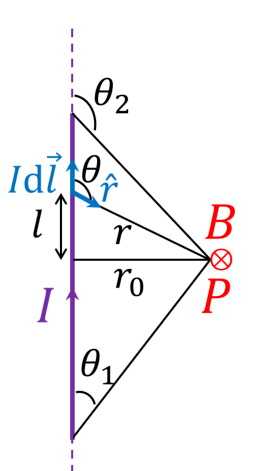
\includegraphics[height=200pt]{m2_finite_wire.png}
\end{column}
\end{columns}
$\theta$ 从电流的去向量起。电流上游的一端 $\theta$ 是锐角，下游的一端是钝角，$\cos\theta_1-\cos\theta_2$ 为正。$a$ 是垂直距离，不是到端点的斜边。
\src{张讲义，PDF124--125，例6.1，式(6.22)--(6.24)；DC5，PDF11--13。}
\end{frame}

\begin{frame}{圆电流环}
\begin{columns}[T,onlytextwidth]
\begin{column}{0.62\textwidth}
半径 $R$ 的圆环，电流 $I$。轴上成对电流元的横向磁场抵消，只留下轴向分量。
\[
 B_z=\frac{\muo I R^2}{2(R^2+z^2)^{3/2}}.
\]
圆心处 $B=\muo I/(2R)$。$z\gg R$ 时
\[
 B_z\simeq\frac{\muo I R^2}{2z^3}=\frac{\muo m}{2\pi z^3}.
\]
磁矩 $\vct m=I\pi R^2\vct e_z$，方向由电流的右手螺旋确定。远处按 $1/z^3$ 衰减，和电偶极子相同。
\end{column}
\begin{column}{0.34\textwidth}
\centering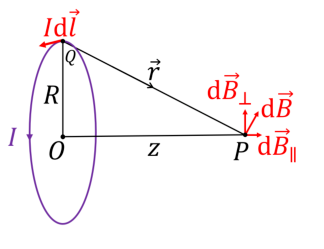
\includegraphics[width=\linewidth]{m2_ring.png}
\end{column}
\end{columns}
轴线公式要求场点在对称轴上。不在轴上时，横向分量不再成对抵消，要改用磁矢势，或在远处用磁偶极子的场。
\src{张讲义，PDF125，例6.2，式(6.27)--(6.31)；DC5，PDF14--16。}
\end{frame}

\begin{frame}{正多边形电流}
正 $N$ 边形通有电流 $I$，中心到每一条边的垂直距离为 $R$。

一条边的两端相对垂足各偏过 $\pi/N$。直导线公式里的两个端角是
\[
 \theta_{1,2}=\frac\pi2\mp\frac\pi N.
\]
代入后，这一条边在中心的场为
\[
 B_{\rm side}=\frac{\muo I}{2\pi R}\sin\frac\pi N.
\]
各边在中心处方向相同，
\[
 \boxed{B=\frac{N\muo I}{2\pi R}\sin\frac\pi N}.
\]
$N\to\infty$ 时 $\sin(\pi/N)\approx\pi/N$，得到 $B\to\muo I/(2R)$，就是半径为 $R$ 的圆电流在圆心的场。

$R$ 是内切圆半径，也就是中心到边的距离，不是中心到顶点的距离。极限若对不上圆电流，先检查用的是不是这个 $R$。
\src{2025秋基础物理学3期中考试A卷-张志财，PDF3，填空4；张讲义例6.1。}
\end{frame}

\begin{frame}{长直螺线管}
理想密绕螺线管，每单位长度 $n$ 匝，电流 $I$。无限长时，$\vct B$ 沿轴向，大小只与到轴的距离有关。

矩形回路的两条长边都在管外时，套住的电流为零，$\vct B$ 不随半径变化。无穷远处场为零，所以管外场为零。再把一条长 $l$ 的长边放进管内：
\[
 B_{\rm in}l=\muo(nl)I,
 \qquad
 \vct B_{\rm in}=\muo nI\,\vct e_z,
 \qquad
 \vct B_{\rm out}=0.
\]
管外这一步用了“无穷远处场为零”。有限长管只在 $L\gg R$、而且远离两个端口时能这样用。半无限长管的轴线上，端口处的场是 $\muo nI/2$。

密绕细螺绕环管内 $B=\muo NI/(2\pi r)$。环很细时 $n=N/(2\pi R)$，与长直螺线管相同。环外的环向场为零。
\src{张讲义，例6.4、例6.8；教材例5.6、例5.8；DC5，PDF35--39。}
\end{frame}

\begin{frame}{厚壁螺线管}
\begin{columns}[T,onlytextwidth]
\begin{column}{0.66\textwidth}
$R_1<s<R_2$ 的壁内有环向电流 $\vct J=J_0\vct e_\phi$，求全空间的 $\vct B$。

把壁拆成半径 $s$、厚度 $\dd s$ 的薄层。这一层的面电流是 $\dd K=J_0\dd s$，相当于 $nI=J_0\dd s$ 的无限长螺线管。螺线管只在内部有场，所以对半径为 $r$ 的场点
\[
 \dd B_z=\begin{cases}
 \muo J_0\dd s,&r<s,\\
 0,&r>s.
 \end{cases}
\]
只有位于场点外侧的电流层有贡献。
\end{column}
\begin{column}{0.30\textwidth}
\centering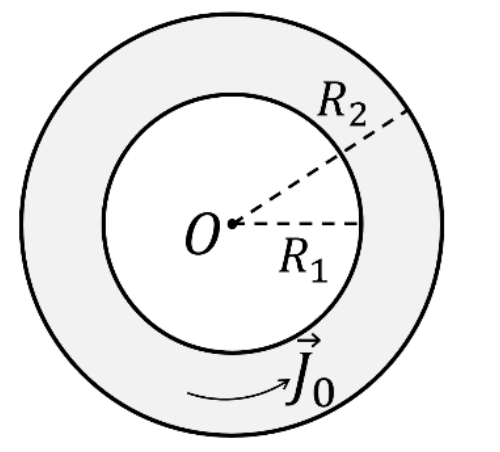
\includegraphics[width=\linewidth]{zhang_solenoid.png}
\end{column}
\end{columns}
积分下限随场点改变：内孔对全部壁积分，壁内只对 $s>r$ 的部分积分，壁外没有贡献。$J_0\dd s$ 的单位是 A/m，和面电流密度相同。
\src{2025秋 A 卷，PDF3，计算1；张讲义例6.4、例6.8。}
\end{frame}

\begin{frame}{壁内外的磁场}
\[
 B_z(r)=\begin{cases}
 \muo J_0(R_2-R_1),&r<R_1,\\[4pt]
 \muo J_0(R_2-r),&R_1<r<R_2,\\[4pt]
 0,&r>R_2.
 \end{cases}
\]
内孔的场是均匀的，大小等于 $\muo$ 乘壁的总面电流密度 $J_0(R_2-R_1)$。壁内场从内边界的值线性降到外边界的零。

在电流区内，$-\dd B_z/\dd r=\muo J_0$，与安培环路定理 $\nabla\times\vct B=\muo\vct J$ 一致。$r=R_1$ 和 $r=R_2$ 上没有额外的面电流，$B_z$ 在这两处都连续。若积分限写成从 $R_1$ 积到 $r$，壁内场会反号，方向就错了。
\src{2025秋 A 卷计算1；配套答案，PDF2。}
\end{frame}

\begin{frame}{磁矢势}
$\nabla\cdot\vct B=0$，而任一矢量的旋度再取散度恒为零，所以存在矢量 $\vct A$，使
\[
 \vct B=\nabla\times\vct A.
\]
$\vct A$ 称为磁矢势。

$\vct A$ 不唯一。换成 $\vct A+\nabla\chi$ 做规范变换之后旋度不变，$\vct B$ 也不变。只给定旋度还定不下 $\vct A$，还要规定它的散度，这就是取规范。

$\vct A$ 沿闭合曲线的积分等于穿过该曲线的磁通：
\[
 \oint_L\vct A\cdot\dd\vct l=\iint_S\vct B\cdot\dd\vct S=\Phi_B.
\]
毕奥--萨伐尔定律先做叉乘再积分。先积$\vct A$只做一次矢量积分，再取旋度。电流产生的 $\vct A$ 大体沿电流方向：直导线的 $\vct A$ 沿导线，圆电流的 $\vct A$ 沿环向。
\src{张讲义，第6.3节，式(6.108)；教材第5.5.1节，式(5.5.1)。}
\end{frame}

\begin{frame}{规范}
库仑规范：$\nabla\cdot\vct A=0$。用 $\nabla\times(\nabla\times\vct A)=\nabla(\nabla\cdot\vct A)-\nabla^2\vct A$，代入 $\nabla\times\vct B=\muo\vct J$，得到
\[
 \nabla^2\vct A=-\muo\vct J.
\]
在直角坐标系里，每个分量都是泊松方程，和电势满足的方程相同。电流稳恒、无穷远处 $\vct A$ 为零时，
\[
 \vct A(\vct r)=\frac{\muo}{4\pi}\iiint\frac{\vct J(\vct r')}{|\vct r-\vct r'|}\,\dd V'.
\]
稳恒条件 $\nabla\cdot\vct J=0$ 保证这个解的散度为零。对它取旋度，就回到毕奥--萨伐尔定律。

洛伦兹规范是
\[
 \nabla\cdot\vct A+\muo\epso\frac{\partial\varphi}{\partial t}=0.
\]
静磁场不随时间变化，上式同样回到 $\nabla\cdot\vct A=0$，方程和解都与库仑规范相同。场随时间变化以后，洛伦兹规范使矢势和电势各自满足波动方程。

e.g.匀强场$\vct B=B\vct e_z$可以取$\vct A=\frac12\vct B\times\vct r$等多种形式。场一直延伸到无穷远时，只要求散度为零，还不能把 $\vct A$ 唯一确定。
\src{张讲义，PDF137--138，式(6.109)--(6.112)；DC5，PDF44--47。静磁场中洛伦兹规范与库仑规范重合。}
\end{frame}

\begin{frame}{静磁场的边值关系}
$\hat{\vct n}$ 从第 1 侧指向第 2 侧。由高斯定理，法向分量连续：
\[
 \hat{\vct n}\cdot(\vct B_2-\vct B_1)=0.
\]
由环路定理，切向分量的跃变由面电流决定：
\[
 \hat{\vct n}\times(\vct B_2-\vct B_1)=\muo\vct K.
\]
这里的 $\vct K$ 是界面上的全部面电流。真空中它就是导线或电流片上的电流。

e.g.无限大均匀面电流两侧是均匀场，大小都是 $\muo K/2$，方向相反，并与电流垂直。密绕长螺线管的管壁可以看成这样的面电流，$K=nI$，管内 $\muo nI$、管外为零，两侧之差正好是 $\muo K$。

\src{由 $\nabla\cdot\vct B=0$ 与 $\nabla\times\vct B=\muo\vct J$ 得到；无限大电流片见教材例5.7，式(5.4.8)。}
\end{frame}

\begin{frame}{洛伦兹力}
\[
 \vct F=q(\vct E+\vct v\times\vct B).
\]
磁力与速度垂直，$\vct F_B\cdot\vct v=0$，不改变动能，只改变方向。

均匀磁场中，平行于 $\vct B$ 的速度分量不变。垂直分量作圆周运动，正、负电荷的回旋方向相反。
\[
 r_c=\frac{mv_\perp}{|q|B},\qquad
 \omega_c=\frac{|q|B}{m},\qquad
 T_c=\frac{2\pi m}{|q|B}.
\]
note：洛伦兹力是相对论下不变的，但是质量等参数需要做相对论变换。
\src{张讲义，第6.4节；教材第5.6节，式(5.6.7)--(5.6.10)；DC5，PDF49、56。}
\end{frame}

\begin{frame}{霍尔效应}
\begin{columns}[T,onlytextwidth]
\begin{column}{0.67\textwidth}
考虑这样的情景情景：电流向右，磁场垂直纸面向里，测得上极板高电势。

电场由高电势指向低电势，所以上极板到下极板的霍尔电场向下。横向达到平衡时，磁力与电场力抵消，
\[
 \vct E_H=-\vct v_d\times\vct B.
\]
由此得到漂移速度 $\vct v_d$ 向右，与电流同向，载流子带正电。若载流子带负电，同样的电流方向要求 $\vct v_d$ 向左，上极板会是低电势。
\end{column}
\begin{column}{0.29\textwidth}
\centering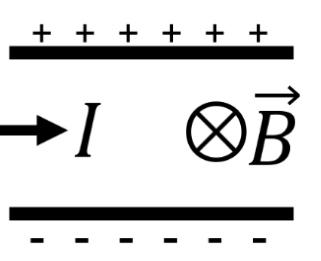
\includegraphics[width=\linewidth]{m2_hall_exam.png}
\end{column}
\end{columns}
单一载流子、厚度 $t$ 沿磁场方向时，
\[
 |U_H|=\frac{IB}{n|q|t},\qquad R_H=\frac{1}{nq}.
\]
$R_H$ 的符号与载流子的符号相同。
\src{2025秋 A 卷，PDF2，选择11；张讲义，PDF138--140；DC5，PDF49--52。}
\end{frame}

\begin{frame}{安培力}
电流元受力
\[
 \dd\vct F=I\dd\vct l\times\vct B,
 \qquad
 \vct F=I\int\dd\vct l\times\vct B.
\]
$\dd\vct l$ 沿电流方向。均匀磁场中，闭合导线的 $\int\dd\vct l=0$，合力为零。合力为零时仍可以有力矩，平面线圈的力矩由磁矩给出。

计算一段导线时，$\vct B$ 取该段所在处的外场。\\
e.g.1面电流自己两侧的场不连续，受力公式里要用两侧的平均值，不能把间断点上的值代进去。
e.g.2两根平行长直导线：电流同向相吸，反向相斥。距离为 $a$ 时，单位长度的力是 $\muo I_1 I_2/(2\pi a)$。
\src{张讲义，式(6.123)；教材第6.1节；DC5，PDF5--7。}
\end{frame}

\begin{frame}{导线受力}
\begin{columns}[T,onlytextwidth]
\begin{column}{0.66\textwidth}
均匀磁场只覆盖闭合导线的一段。沿电流方向，入场点为 $A$，出场点为 $B$。场外 $\vct B=0$，总力只来自场内这一段：
\[
 \vct F=I\int_A^B\dd\vct l\times\vct B
 =I(\vct r_B-\vct r_A)\times\vct B.
\]
若$\vct B$ 均匀，可以把它提出积分。积分 $\int_A^B\dd\vct l$ 只取决于两端，与场内导线弯曲形状无关。

两交点间距为 $w$，磁场垂直于导线所在平面时，$F=IBw$。
\end{column}
\begin{column}{0.30\textwidth}
\centering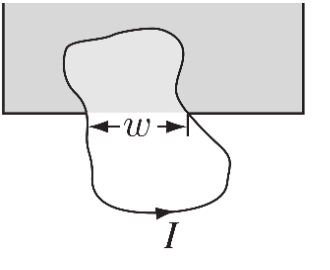
\includegraphics[width=\linewidth]{m2_force_exam.png}
\end{column}
\end{columns}
整环都在同一均匀场中时，$\vct r_B=\vct r_A$，合力为零。
\src{2025秋 A 卷，PDF2--3，选择12；DC5，PDF7，半圆导线受力。}
\end{frame}

\begin{frame}{磁矩}
平面线圈的面积为 $S$，法向与电流成右手关系：
\[
 \vct m=IS\vct n.
\]
均匀外场中，闭合线圈合力为零，力矩和能量为
\[
 \vct\tau=\vct m\times\vct B,
 \qquad
 U=-\vct m\cdot\vct B.
\]
电流保持不变时用这个能量。$\vct m$ 与 $\vct B$ 同向时能量最低，反向时最高。

线圈很小，磁矩不随位置改变，且线圈所在处没有电流时，磁矩受力为
\[
 \vct F=\nabla(\vct m\cdot\vct B).
\]
它和 $(\vct m\cdot\nabla)\vct B$ 相同。线圈所在处有电流时，回到安培力重新积分。

远处的场和电偶极子对应。磁矩 $\vct m$ 在 $r$ 远大于线圈尺寸处，
\[
 \vct B=\frac{\muo}{4\pi r^3}\bigl[3(\vct m\cdot\hat{\vct r})\hat{\vct r}-\vct m\bigr].
\]
\src{张讲义，式(6.121)--(6.122)，例6.10；教材式(6.1.9)、(6.1.10)。}
\end{frame}

\begin{frame}{e.g.3.1旋转带电圆盘}
半径 $R$ 的圆盘均匀带电 $q$，以角速度 $\vct\omega=\omega\vct e_z$ 绕轴转动。面密度 $\sigma=q/(\pi R^2)$。

半径 $r$、宽度 $\dd r$ 的环带，电量 $\dd q=\sigma\,2\pi r\dd r$。转一圈的时间是 $2\pi/\omega$，对应的电流
\[
 \dd I=\sigma\omega r\,\dd r.
\]
$q>0$ 时电流沿转动方向，$q<0$ 时相反。

该环在圆心的场用圆电流公式，
\[
 \dd B_z=\frac{\muo\dd I}{2r}=\frac{\muo\sigma\omega}{2}\dd r.
\]
环带电量随 $r$ 增大，圆电流中心场中的 $1/r$ 正好抵消，等宽环带的贡献相同。
\[
 B_z=\frac{\muo\sigma\omega R}{2}=\frac{\muo q\omega}{2\pi R},
 \qquad
 \vct B_O=\frac{\muo q}{2\pi R}\vct\omega.
\]
总电荷和角速度固定时，中心磁场按 $1/R$ 减小。这个 $\vct B_O$ 是盘自己在圆心的场，不是外加场。
\src{张讲义习题6.10(1)；教材习题6.6；第六周作业，6.6。}
\end{frame}

\begin{frame}{e.g.3.2旋转带电圆盘}
每一环带的磁矩是电流乘环面积，方向都沿 $\vct\omega$（$q>0$）：
\[
 \dd m=\pi r^2\dd I=\pi\sigma\omega r^3\dd r.
\]
\[
 \vct m=\pi\sigma\omega\int_0^R r^3\dd r\,\vct e_z
 =\frac{q R^2}{4}\vct\omega.
\]
均匀外场 $\vct B_{\rm ext}$ 平行于盘面时，
\[
 \vct\tau=\vct m\times\vct B_{\rm ext},
 \qquad
 |\tau|=\frac{|q|\omega R^2 B_{\rm ext}}{4}.
\]
磁矩的被积函数带 $r^3$，外圈贡献大。中心磁场的被积函数是 $\dd r$，各圈一样。两个积分的权重不同，不能用中心磁场乘总面积去写磁矩。

力矩公式里的 $\vct B_{\rm ext}$ 是外加的均匀场。盘自己的场对总力矩没有贡献。
\src{张讲义习题6.10(2)，参考答案 PDF216；教材习题6.6。}
\end{frame}

\begin{frame}{磁化强度}
磁化强度是单位体积内分子磁矩的矢量和，
\[
 \vct M=\frac{\dd\vct m}{\dd V}.
\]
单位是 A/m。分子电流排列整齐以后，宏观上相当于一组磁化电流。$\hat{\vct n}$ 指向介质外部时，
\[
 \vct J'=\nabla\times\vct M,
 \qquad
 \vct K'=\vct M\times\hat{\vct n}.
\]
$\vct J'$ 的单位是 A/m$^2$，$\vct K'$ 的单位是 A/m。

\begin{columns}[T,onlytextwidth]
\begin{column}{0.48\textwidth}
\centering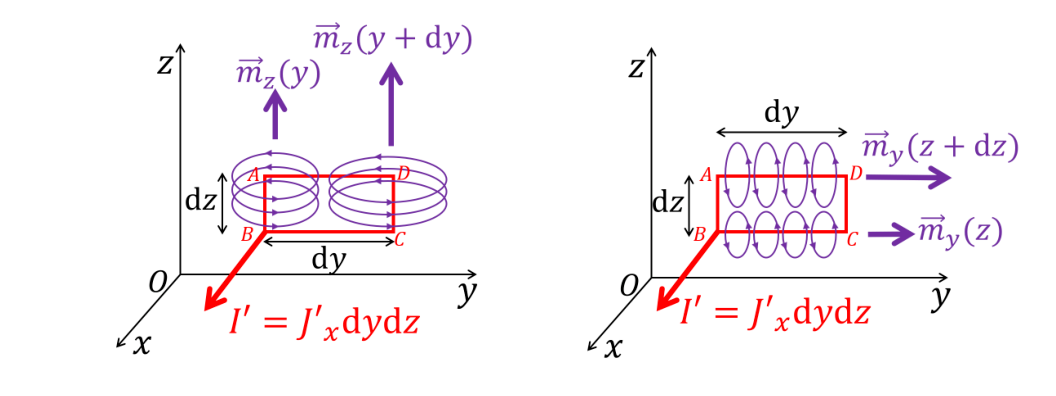
\includegraphics[width=0.92\linewidth]{m2_bound_bulk.png}
\end{column}
\begin{column}{0.48\textwidth}
$\vct M$ 均匀时，内部相邻分子电流首尾抵消，$\vct J'=0$，表面仍可以有 $\vct K'$。$\vct M$ 沿外法向没有贡献；平行于表面的分量留下环向面电流。
\end{column}
\end{columns}
磁化电流激发磁场、也受磁场作用，算法与传导电流相同。但是它不伴随电荷的宏观迁移，不会产生焦耳热。
\src{张讲义，式(7.2)、(7.12)；教材式(6.2.5)、(6.2.6)；DC6，PDF21--24。}
\end{frame}

\begin{frame}{磁场强度}
总电流是传导电流加磁化电流，$\nabla\times\vct B=\muo(\vct J_0+\nabla\times\vct M)$。定义
\[
 \vct H=\frac{\vct B}{\muo}-\vct M,
 \qquad
 \vct B=\muo(\vct H+\vct M),
\]
则
\[
 \oint_L\vct H\cdot\dd\vct l=I_{0,\rm enc},
 \qquad
 \nabla\times\vct H=\vct J_0.
\]
右端只有传导电流。这个定义不要求介质是线性的。$\vct H$ 和 $\vct M$ 的单位都是 A/m。

各向同性线性介质中
\[
 \vct M=\chi_m\vct H,
 \qquad
 \vct B=\mu\vct H,
 \qquad
 \mu=\mu_r\muo=\muo(1+\chi_m).
\]
这里的 $\vct H$ 是介质内的总场。对称性允许画安培环路时，先由传导电流求 $\vct H$，再由 $\vct B=\mu\vct H$ 求 $\vct B$。

永磁体的 $\vct M$ 由磁化历史给定，$\vct B=\mu\vct H$未必成立。
\src{张讲义，式(7.16)--(7.21)、(7.35)--(7.38)；教材式(6.3.4)、(6.3.5)。}
\end{frame}

\begin{frame}{与静电场的对应}
$\vct H$ 对应 $\vct E$，$\vct B$ 对应 $\vct D$。本构关系
\[
 \vct D=\epso\vct E+\vct P
 \quad\longleftrightarrow\quad
 \vct B=\muo\vct H+\muo\vct M,
\]
所以 $\vct P$ 对应 $\muo\vct M$。线性介质里 $\vct D=\varepsilon\vct E$ 对应 $\vct B=\mu\vct H$，$\varepsilon$ 对应 $\mu$。

这个对应来自定义，有传导电流时仍然成立。$\nabla\times\vct H=\vct J_0$ 只说明该区域不能写磁标势，求 $\vct H$ 改用环路定理。没有传导面电流时，切向 $\vct H$ 连续，对应切向 $\vct E$ 连续；法向 $\vct B$ 始终连续，对应没有自由面电荷时的法向 $\vct D$。
\src{教材第6.8节，表6.2：$\vct H\!\leftrightarrow\!\vct E$，$\vct B\!\leftrightarrow\!\vct D$，$\muo\vct M\!\leftrightarrow\!\vct P$。}
\end{frame}

\begin{frame}{磁介质的边值关系}
$\hat{\vct n}$ 从介质 1 指向介质 2。界面上的传导面电流为 $\vct K_0$ 时，
\[
 \hat{\vct n}\cdot(\vct B_2-\vct B_1)=0,
 \qquad
 \hat{\vct n}\times(\vct H_2-\vct H_1)=\vct K_0.
\]
法向 $\vct B$ 连续，和有没有介质无关。切向 $\vct H$ 的跃变只由传导面电流决定，磁化面电流已经吸收进 $\vct H$ 的定义里。

没有传导面电流时，$B_n$ 连续，$H_t$ 连续。线性介质中 $\mu_1 H_{1n}=\mu_2 H_{2n}$。$\vct B$ 与法线的夹角满足
\[
 \frac{\tan\theta_2}{\tan\theta_1}=\frac{\mu_2}{\mu_1}.
\]
按 $\vct H$ 对应 $\vct E$、$\mu$ 对应 $\varepsilon$，电介质折射公式里 $\varepsilon$ 换成 $\mu$。$\mu$ 大的一侧，磁感应线贴近界面。

\src{张讲义，第7.4节，式(7.43)、(7.46)、(7.48)；教材第6.5节；DC6，PDF43--45。}
\end{frame}

\begin{frame}{均匀磁化圆柱}
\begin{columns}[T,onlytextwidth]
\begin{column}{0.70\textwidth}
无限长圆柱内 $\vct M=M\vct e_z$ 为常矢量，柱外真空，没有传导电流，也没有外加场。
\[
 \vct J'=\nabla\times\vct M=0.
\]
侧面 $\hat{\vct n}=\vct e_r$，
\[
 \vct K'=\vct M\times\vct e_r=M\vct e_\phi.
\]
这就是面电流密度 $nI=M$ 的理想螺线管，所以
\[
 \vct B_{\rm in}=\muo\vct M,\qquad
 \vct B_{\rm out}=0,\qquad
 \vct H=0.
\]
\end{column}
\begin{column}{0.26\textwidth}
\centering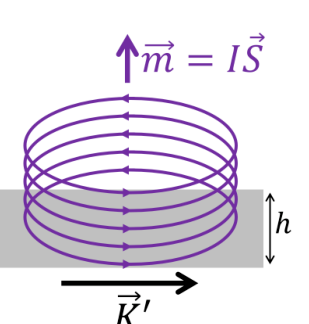
\includegraphics[width=\linewidth]{m2_bound_surface.png}
\end{column}
\end{columns}
管内 $\vct B$ 与同样 $nI$ 的真空螺线管相同，但螺线管内是有 $\vct H$、没有 $\vct M$，永磁棒内是有 $\vct M$、没有 $\vct H$。按 $\vct H$ 对应 $\vct E$，无限长样品的退磁场为零，$\vct H_{\rm in}=0$，同样得到 $\vct B_{\rm in}=\muo\vct M$。

\src{张讲义例7.3；教材例6.4；DC6，PDF24--25、例12。}
\end{frame}

\begin{frame}{螺线管中的磁介质}
\begin{columns}[T,onlytextwidth]
\begin{column}{0.66\textwidth}
无限长螺线管内充满各向同性线性介质，每单位长度 $n$ 匝，传导电流 $I$。

环路套住的是传导电流，
\[
 H_{\rm in}=nI,\qquad H_{\rm out}=0.
\]
再由本构关系，
\[
 M=\chi_m nI,\qquad
 B_{\rm in}=\mu nI=\mu_r\muo nI.
\]
顺磁质 $\chi_m>0$，磁化电流与传导电流同向，管内 $\vct B$ 比真空大。逆磁质相反。
\end{column}
\begin{column}{0.30\textwidth}
\centering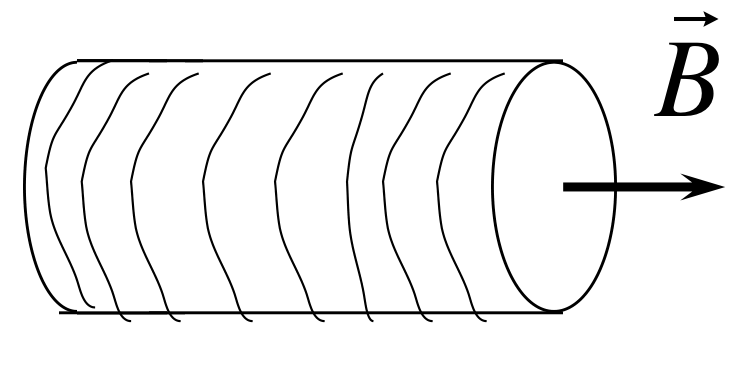
\includegraphics[width=\linewidth]{m2_filled_solenoid.png}
\end{column}
\end{columns}
\src{张讲义例7.2；教材例6.6；DC6，PDF25--27。}
\end{frame}

\begin{frame}{载流介质圆柱}
无限长圆柱半径 $R$、磁导率 $\mu$，内部均匀传导电流 $\vct J_0=J_0\vct e_z$，柱外真空。环路定理先给出 $\vct H$，它只由 $\vct J_0$ 决定。
\begin{columns}[T,onlytextwidth]
\begin{column}{0.78\textwidth}
\[
 H_\phi=\begin{cases}J_0 r/2,&r<R,\\J_0 R^2/(2r),&r>R,\end{cases}
 \qquad
 B_\phi=\begin{cases}\mu H_\phi,&r<R,\\\muo H_\phi,&r>R.\end{cases}
\]
柱内 $\vct M=\chi_m J_0 r\,\vct e_\phi/2$，因此
\[
 \vct J'=\chi_m J_0\vct e_z,\qquad
 \vct K'=-\frac{\chi_m J_0 R}{2}\vct e_z.
\]
体磁化电流与面磁化电流之和为零。柱外 $\vct B$ 与真空中同一传导电流的场相同。
\end{column}
\begin{column}{0.18\textwidth}
\centering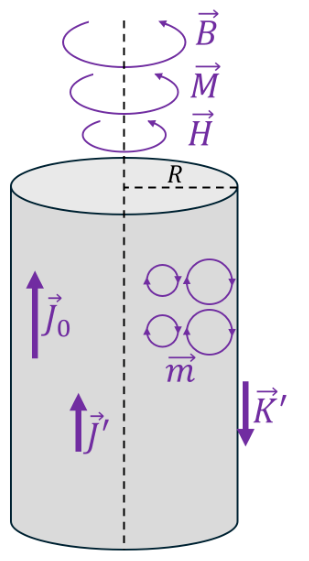
\includegraphics[height=130pt]{m2_magnetic_cylinder.png}
\end{column}
\end{columns}
柱面没有传导面电流，$H_\phi$ 连续。$\mu\neq\muo$ 时 $B_\phi$ 跃变。$\chi_m=\mu_r-1$，逆磁质的 $\vct J'$ 与 $\vct J_0$ 反向。
\src{张讲义例7.1，式(7.23)--(7.27)；DC6，PDF28--29。}
\end{frame}

\begin{frame}{磁化球}
均匀磁化球的 $\vct M$ 是常矢量，球外真空，没有传导电流。按 $\vct H$ 对应 $\vct E$、$\muo\vct M$ 对应 $\vct P$，均匀极化球的退极化场换成
\[
 \vct H_{\rm in}=-\frac{\vct M}{3},\qquad
 \vct B_{\rm in}=\frac{2\muo}{3}\vct M.
\]
总磁矩 $\vct m=(4\pi R^3/3)\vct M$。球外是这个磁矩的偶极场。

$\vct H_{\rm in}$ 与 $\vct M$ 反向，叫做退磁场。长圆柱里退磁场为零，球里是 $-\vct M/3$，很扁的盘接近 $-\vct M$。代换时用 $\vct M$ 对应 $\vct P/\epso$，分母里不再写 $\muo$。写成 $-\muo\vct M/3$ 就多了一个 $\muo$。
\src{张讲义习题7.2；教材第6.8节。球外偶极场与圆电流远场同一形式。}
\end{frame}

\begin{frame}{磁介质球}
线性介质球放在均匀外场 $\vct H_0$ 中，球外为真空，$\vct B_0=\muo\vct H_0$。静电场中介质球的内场是
\[
 \vct E_{\rm in}=\frac{3\epso}{\varepsilon+2\epso}\vct E_0.
\]
按 $\vct H$ 对应 $\vct E$、$\muo$ 对应 $\epso$、$\mu$ 对应 $\varepsilon$，
\[
 \boxed{\vct H_{\rm in}=\frac{3\muo}{\mu+2\muo}\vct H_0},
 \qquad
 \vct B_{\rm in}=\frac{3\mu}{\mu+2\muo}\vct B_0.
\]
\[
 \vct M=\frac{3(\mu-\muo)}{\mu+2\muo}\vct H_0.
\]
先得到 $\vct H_{\rm in}$，再乘 $\mu$ 得到 $\vct B_{\rm in}$。分子上是 $3\mu$，也就是 $3\mu_r\vct B_0/(\mu_r+2)$。

$\mu=\muo$ 时球不磁化。$\mu$ 很大时球内 $\vct H$ 趋于零，磁感应线被吸进球内。
\src{教材例6.13，由例2.8按 $\vct H$ 对应 $\vct E$ 代换；张讲义习题7.3。}
\end{frame}

\begin{frame}{顺磁质与铁磁质}
\begin{columns}[T,onlytextwidth]
\begin{column}{0.66\textwidth}
逆磁质的分子没有固有磁矩，外场感应出的磁矩与外场反向，$\chi_m<0$，$\mu_r<1$，数值通常比 $1$ 只小百万分之一量级。

顺磁质有固有磁矩，外场使它们趋向与外场平行，热运动把取向打乱，$\chi_m>0$ 但仍然远小于 $1$。

铁磁质里磁矩成畴。外场使畴壁移动、磁矩转向，可以达到饱和，去掉外场后还留下剩磁。$\vct B$ 与 $\vct H$ 不是单值的线性关系，还取决于磁化历史。回线包围的面积对应一个循环里损耗的能量。矫顽力大的是硬磁，用来做永磁体；矫顽力小的是软磁，用来做变压器铁芯。
\end{column}
\begin{column}{0.30\textwidth}
\centering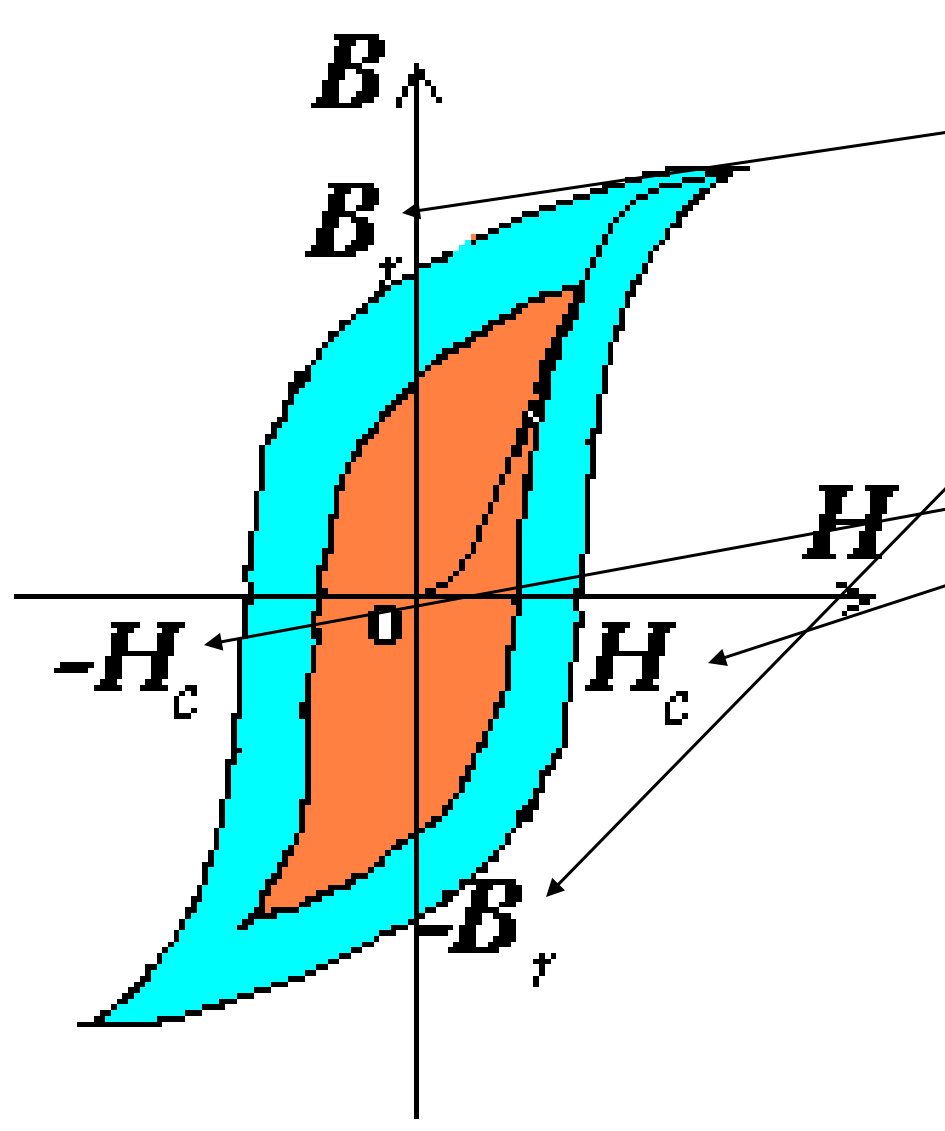
\includegraphics[height=175pt]{m2_hysteresis.png}
\end{column}
\end{columns}
\src{张讲义，PDF145--147、153；DC6，PDF15--20、55--62。}
\end{frame}

\begin{frame}{磁路}
磁感应线集中在铁芯里形成的通路叫做磁路。$\mu\gg\muo$ 时，漏到空气中的磁通可以忽略。沿一条磁路，磁通 $\Phi_B=BS$ 近似不变。

对闭合磁路，安培环路定理写成
\[
 NI=\oint\vct H\cdot\dd\vct l=\Phi_B\sum_i R_{m,i},
 \qquad
 R_m=\frac{l}{\mu S}.
\]
$NI$ 叫磁动势，$R_m$ 叫磁阻。磁动势等于各段磁势降 $\Phi_B R_m$ 之和。截面和材料分段均匀时，第 $i$ 段用该段的 $l_i$、$\mu_i$、$S_i$。

这是和直流电路的对应：磁通对电流，磁动势对电动势，磁阻 $l/(\mu S)$ 对电阻 $l/(\sigma S)$。这里 $\vct H$ 对电路中的电场，$\vct B$ 对电流密度，$\mu$ 对电导率。

介质球用的是另一套：$\vct H$ 对 $\vct E$，$\vct B$ 对 $\vct D$，$\mu$ 对 $\varepsilon$。磁路里 $\vct B$ 对的是电流密度，磁阻用 $l/(\mu S)$。

铁芯的 $\mu$ 要远大于 $\muo$，气隙要窄，否则漏磁不能忽略。软磁近似把 $\mu$ 当成常数。
\src{教材第6.7节，式(6.7.11)、(6.7.12)；DC6，第6.4节。}
\end{frame}

\begin{frame}{带气隙的磁路}
铁芯长度 $l$、截面积 $S$、磁导率 $\mu$，线圈 $N$ 匝、电流 $I$。气隙长度 $d$，气隙窄，截面仍按 $S$ 算，漏磁忽略。
\[
 NI=\Phi_B\left(\frac{l}{\mu S}+\frac{d}{\muo S}\right).
\]
没有气隙时
\[
 \Phi_B=\frac{\mu S\,NI}{l}.
\]
磁通减到这个值的一半时，
\[
 d=\frac{\muo}{\mu}\,l.
\]
铁芯磁阻是 $l/(\mu S)$，气隙磁阻是 $d/(\muo S)$。$\mu/\muo$ 常在 $10^3$ 以上，气隙只有铁芯长度的千分之一，两段磁阻就一样大，磁通主要由这段短气隙决定。

气隙里 $H$ 大约是铁芯里的 $\mu/\muo$ 倍，$\vct B$ 则两侧接近。
\src{教材第6.7.2节，图6.24及日光灯镇流器一例；DC6，例13。}
\end{frame}
